%
% Anatomía de PANs, presentación de cifrados que preservan el formato.
% Proyecto Lovelace.
%

\section{Anatomía de un número de tarjeta}

\begin{frame}{Anatomía de un número de tarjeta}
  {Sobre el PAN}
  Un número de tarjeta (PAN, por sus siglas en inglés), se compone por tres
  partes:
  \begin{figure}[H]
    \begin{center}
      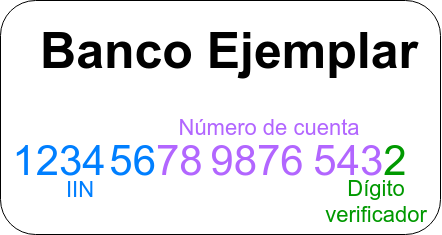
\includegraphics[width=0.5\linewidth]{diagramas/tarjeta.png}
    \end{center}
  \end{figure}

  Los números están regidos por el ISO/IEC-7812.
  La longitud del número de tarjeta puede ir desde 12 hasta 19 dígitos.
\end{frame}

\begin{frame}{Anatomía de un número de tarjeta}
  {Sobre el MII}
  El primer dígito de la tarjeta se refiere al
  \textit{Major Industry Identifier} (MII). La relación entre dígitos e
  industrias es la siguiente:
  \begin{itemize}
    \item 1, 2: Aerolíneas
    \item 3: Viajes y entretenimiento (American Express, JBC)
    \item 4, 5: Bancos e industria financiera (Visa, Electron, Mastercard)
    \item 6: Comercio (Discover, Laser, China UnionPay)
    \item 7: Industria petrolera
    \item 8: Telecomunicaciones
    \item 9: Asignación nacional
  \end{itemize}
\end{frame}

\begin{frame}{Anatomía de un número de tarjeta}
  {Sobre el IIN}
  El \textit{Issuer Identification Number} (IIN) comprende los primeros
  6 dígitos, incluyendo el MII. El IIN puede proveer los siguientes datos:
  \begin{itemize}
    \item Banco emisor de la tarjeta
    \item Tipo de la tarjeta (crédito o débito)
    \item Marca de la tarjeta (Visa, MasterCard, Discover)
    \item Nivel de la tarjeta (Clásica, Gold, Black)
  \end{itemize}
\end{frame}

\begin{frame}{Anatomía de un número de tarjeta}
  {Sobre el IIN}
  La base de datos BINDB proveé información cuando se ingresa un BIN%
  \footnote{\textit{Bank Identifier Number}} válido.
  Permite solo 10 consultas gratuitas por computadora.
  \begin{figure}[H]
    \begin{center}
      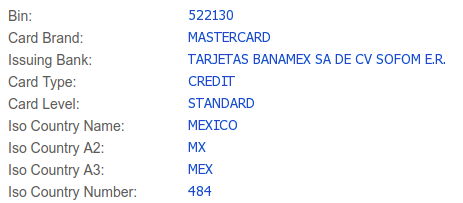
\includegraphics[width=0.75\linewidth]{diagramas/bindb.png}
    \end{center}
  \end{figure}
\end{frame}

\begin{frame}{Anatomía de un número de tarjeta}
  {Sobre el número de cuenta}
  Los dígitos que siguen al IIN, excepto el último, son el número de cuenta.
  El número de cuenta puede variar, pero máximo comprende 12 dígitos, por lo que
  cada emisor tiene $10^{12}$ posibles números de cuenta.
\end{frame}

\begin{frame}{Anatomía de un número de tarjeta}
  {Sobre el dígito verificador}
  El dígito verificador se obtiene de la siguiente manera:
  \begin{enumerate}
    \item Comenzando desde la derecha, se obtiene el doble de cada segundo
      dígito. Si el producto es mayor a $9$, se suman sus dígitos.
      \begin{figure}[H]
        \begin{center}
          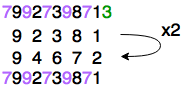
\includegraphics[width=0.3\linewidth]{diagramas/luhn_1.png}
        \end{center}
      \end{figure}
    \item Se suman todos los dígitos.
    \item Se multiplica la suma por $9 \mod  10$.
      \begin{figure}[H]
        \begin{center}
          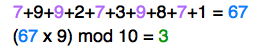
\includegraphics[width=0.5\linewidth]{diagramas/luhn_2.png}
        \end{center}
      \end{figure}
  \end{enumerate}
  El proceso para obtener el dígito verificador es conocido como el algoritmo de
  Luhn.
\end{frame}
